\documentclass[portugues, 12pt, a4paper]{article}
\usepackage[
  top=2cm,
  bottom=2cm,
  left=3cm,
  right=1.5cm,
  headheight=17pt, % as per the warning by fancyhdr
  includehead,includefoot,
  heightrounded, % to avoid spurious underfull messages
]{geometry} 

\usepackage[utf8]{inputenc}
\usepackage[brazil]{babel}
\usepackage{fancyhdr}
\usepackage{cite}
\usepackage{booktabs}
\usepackage{hyperref}
\usepackage{mathtools}
\usepackage{subfigure}
\usepackage{xparse}
\usepackage{graphicx}
\usepackage{nccmath}
\usepackage{amsmath}
\usepackage{amssymb}
\usepackage{pifont}
\usepackage[numbers]{natbib}
\usepackage{svg}
\usepackage{multirow}
\usepackage{makecell}

\RequirePackage{logos}
% Note that due to the logos package setup, you can call any logo definition in the logos folder.
% The restriction is to have a <NAME>.logo file which contains a \@logo<NAME> macro that typesets the logo.

% Load the logos
\getlogo{IC3D}
\getlogo{UNICAMP}

\def\logos{
  \noindent
  \begin{center}%
  \begin{tabular}{ccc}%
    \setlogo{UNICAMP}%
    &%
    \begin{minipage}{.6\textwidth}%
      \centering%
      \textbf{Universidade Estadual de Campinas} \\%
      \textbf{Instituto de Computa\c{c}\~ao} \\%
    \end{minipage}%
    &%
    \setlogo[Instituto de Computa\c{c}\~ao]{IC3D}%
  \end{tabular}%
  \end{center}%
}

\newcommand{\cmark}{\ding{51}}

\fancypagestyle{firststyle}
{
	\fancyhf{}
	\chead{\logos}
	\cfoot{\thepage}
}

\fancypagestyle{secondstyle}
{
	\fancyhf{}
	\renewcommand{\headrulewidth}{0pt}
	\chead{}
	\cfoot{\thepage}
}

\begin{document}
\thispagestyle{firststyle}
\hfill \newline \newline \newline \newline
\begin{center}
\textbf{Projeto de Mestrado: Proposta de arquitetura para soluções de IA envolvendo métricas de Fairness e AI Explainability}
\end{center}
\hfill \newline \newline
\textbf{Aluno:} Thales Eduardo Nazatto \newline
\textbf{Orientadora:} Cecília Mary Fischer Rubira \newline
\textbf{Co-Orientador:} Leonardo Montecchi \newline \newline \newline

\begin{center}\textbf{Resumo}\end{center}

Este projeto de Mestrado possui o objetivo de contribuir com o tema de Inteligência Artificial (IA) do ponto de vista da Engenharia de Software, visto que o uso de IA envolvendo grandes volumes de dados vem crescendo conforme nossa sociedade migra processos manuais de trabalho para soluções digitais e necessita de tomadas de decisão mais rápidas e assertivas. Entretanto, as métricas usadas inicialmente para definir a eficácia de um algoritmo se mostraram limitadas devido a barreiras éticas e legais, resultando em vieses que refletem a sociedade de maneira que não era esperada pelos desenvolvedores da solução. Desta forma, a elaboração de diretrizes arquiteturais para uma aplicação de IA incluir conceitos de Explainability AI e métricas de Fairness pode ajudar neste problema. Desenvolvendo componentes, documentando métodos e ferramentas, e realizando estudos de caso, é esperado que este problema seja controlado e facilite o desenvolvimento de softwares com o uso responsável de dados. \newline \newline \newline

\begin{center}\textbf{Abstract}\end{center}

This Master's Degree project aims to contribute to the theme of Artificial Intelligence (AI) from the Software Engineering point of view, since the use of AI involving large volumes of data has been growing as our society migrates manual work processes to digital solutions and needs faster and more assertive decision making. However, the metrics used initially to define the effectiveness of an algorithm proved to be limited due to ethical and legal barriers, resulting in biases that reflect society in a way that was not expected by the solution developers. Thus, the elaboration of architectural guidelines for an AI application including concepts of Explainability AI and Fairness metrics can help with this problem. By developing components, documenting methods and tools, and making case studies, it is expected that this problem will be controlled and facilitate software development with the responsible use of data.
\newpage

\thispagestyle{secondstyle}
\newgeometry{top=2cm,bottom=2cm,left=3cm,right=1.5cm, footskip=5mm}

\section{Introdução}

Técnicas de Inteligência Artificial e Aprendizado de Máquina já são utilizadas há bastante tempo no ramo da Computação. Ramos como robótica e jogos são grandes exemplos, dada a necessidade nos mesmos de automatizar comportamentos que seriam tidos como triviais para um ser humano. Entretanto, nos últimos anos ocorreu um crescimento no uso dessas tecnologias em aplicações tradicionais, com previsão de US\$ 57 bilhões em investimentos em 2021, 480\% maior em relação a 2017~\citep{Deloitte_2018}. No Brasil, o número de empresas de IA aumentou de 120 em 2018 para 206 em 2020~\citep{CIO_2021}.

Isso se mostra possível devido a grande quantidade de dados processada diariamente pelas empresas, que coletam estatísticas toda vez que um usuário acessa suas aplicações. Com esses dados, podem traçar diferentes perfis e usar soluções de IA para ter tomadas de decisão mais assertivas com o objetivo de melhorar a experiência de usuário e corrigir problemas. Porém, muitas dessas soluções foram projetadas sem pensar em governança de dados como requisito de projeto, e se mostram ineficientes quando ela é tratada em consideração.

Governança de dados é um tema que entrou em evidência recentemente em países como o Brasil: Iniciativas como a LGPD - Lei Geral de Proteção de Dados \citep{LGPD_2021}, de 14 de agosto de 2018, mostram como as aplicações e seus dados possuem cada vez mais influência na sociedade moderna. E nesse ponto muitas aplicações de IA falham: muitas implementações foram implementadas como \textit{black boxes}, onde o determinante para estabelecer a confiança no modelo implementado é sua entrada e sua saída.

Um outro efeito colateral dessa estratégia é a exposição de vieses que, embora sejam vistos como não-intencionais pelos desenvolvedores por ter a possibilidade de ser um \textit{outlier} no modelo treinado, refletem preconceitos escancarados da sociedade atual. Uma entrada de dados enviesada resulta em um algoritmo que realiza discriminações em sua classificação~\citep{Buolamwini_2018}, e uma vez que as métricas utilizadas para medir a qualidade de um modelo \textit{black box} são geralmente baseadas em acurácia, precisão e recall, discriminações não são facilmente percebidas por tais métricas. Ao mesmo tempo, um modelo \textit{black box} pode ter uma alta dependência de poucos dados, determinando problemas de acoplamento. Para resolver este problema, é possível que a criação de um novo modelo seja uma melhor opção que realizar a correção em apenas parte dele.

Devido a esses tipos de problemas, o termo \textit{Explainable AI} (XAI) ganha força para envolver o desenvolvimento de uma IA que seja acurada e simultaneamente transparente. Como IA possui diversos tipos de métodos diferentes para enquadrar diversos tipos de dados, o mesmo acaba se aplicando em Explainable AI, podendo enquadrar em diversos tipos de dados~\citep{Sundararajan_2017}, ou dados específicos como imagens~\citep{Kapishnikov_2019} e tabelas~\citep{Maleki_2013}. No mesmo tema, é possível estabelecer métricas para determinar o quão o modelo está preparado para dados sensíveis \citep{Begley_2021}, termo que é conhecido como \textit{Fairness}.

Como o objetivo em XAI é fazer com que os resultados alcançados pela solução de IA sejam compreendidos por humanos, é possível considerar este fato como requisito no design de uma solução de IA, fazendo com que a mesma seja reusável e testável. O objetivo deste projeto de mestrado é estabelecer uma arquitetura para desenvolvimento de uma solução já baseada nestes conceitos, permitindo a criação de um algoritmo confiável e capaz de ser mantido por vários desenvolvedores.

O restante desse documento se organiza da seguinte forma: a Seção 2 descreve os conceitos que irão ser abordados neste projeto; a Seção 3 mostra trabalhos semelhantes; a Seção 4 enumera as resultados esperados desse projeto; a Seção 5 discute desafios a serem enfrentados e, finalmente, a Seção 6 estabelece o cronograma do projeto.

\section{Conceitos Abordados}

\subsection{AI Explainability}

\textit{AI Explainability} é um conceito em IA que propõe a criação de um conjunto de técnicas de Aprendizado de Máquina (ou Machine Learning/ML) que produz modelos mais explicáveis, mantendo qualidade em suas métricas, e permite que os humanos entendam, confiem e gerenciem aplicações baseadas em IA. XAI também absorve conceitos das Ciências Sociais e considera a psicologia da explicação~\citep{Arrieta_2020}. Um algoritmo de ML explicável precisa não apenas mostrar tomadas de decisão, mas também mostrar o processo que o levou ao tomar tal decisão, de modo que seja compreensível e transparente para humanos.

\begin{figure}[h]
\centering
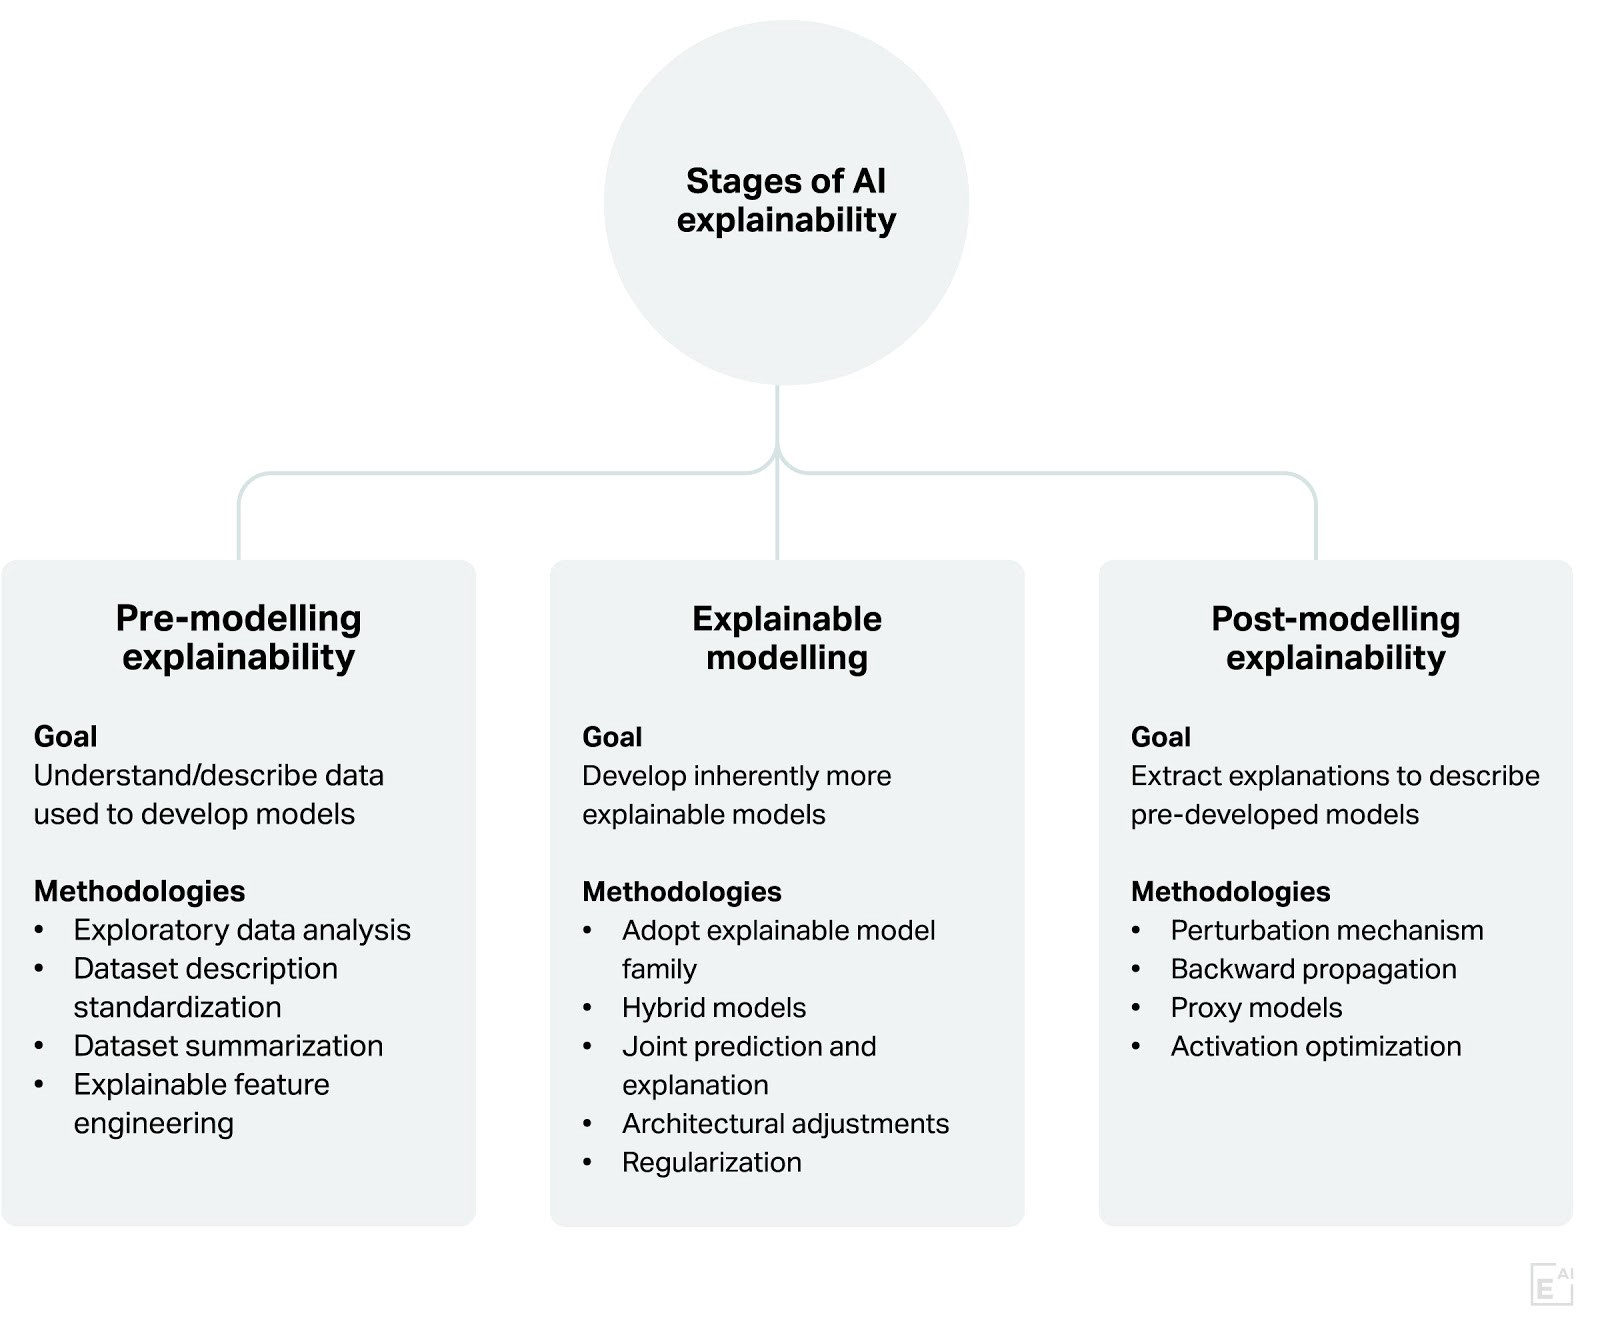
\includegraphics[scale=0.2]{images/phases.jpeg}
\caption {Fases de um processo baseado em IA explicável.}
\label{fig:StagesExplainableAI}
\end{figure}

Conforme ilustrado na Figura \ref{fig:StagesExplainableAI}, o um processo baseado em IA explicável pode ser classificado em 3 fases:

\begin{itemize}
\item \textbf{\textit{Pre-Modelling Explainability}:} Esta fase se caracteriza por obter explicações no conjunto de dados usado para treino e validação, tendo como principal motivação o fato do comportamento de um modelo depender muito dos dados que o alimentam. Análises e visualizações dos dados, ou mesmo através de documentações do conjunto de dados se enquadram neste estágio.~\citep{Khalegi_2019_Pre} 
\item \textbf{\textit{Explainable Modelling}:} Esta fase se caracteriza por obter explicações por modelos considerados transparentes (ver adiante). Ao adotar modelos deste tipo, ele já pode ser considerado como explicável por um humano. Também é possível obter a explicação através de regularizadores, ou adotar abordagens onde explicação e resultado sejam obtidos simultaneamente, sejam via junção de dados ou sendo intrínseco a arquitetura do modelo.~\citep{Khalegi_2019}
\item \textbf{\textit{Post-Modelling Explainability}:} Também chamada de \textit{Post-hoc Explainability} e onde a maioria dos trabalhos disponíveis baseados em XAI tenta focar, esta fase se dedica a explicar modelos desenvolvidos anteriormente, ou modelos que não são considerados como transparentes. Pode-se explicar um modelo por métodos como árvores de decisão e estimativas como valores de Shapley e propagação inversa.~\citep{Khalegi_2019_Post}
\end{itemize}

Entretanto, estas 3 fases não necessariamente são executadas de maneira sequencial: Por ser realizada no conjunto de dados e não no modelo, a fase de \textit{Pre-modelling Explainability} pode ser opcional, e a aplicação das fases de \textit{Explainable Modelling} e \textit{Post-Modelling Explainability} e seus métodos dependem exclusivamente se o modelo é classificado como transparente ou não, e tal critério é determinado pela adoção de uma (ou mais) das seguintes características~\citep{Arrieta_2020}:

\begin{itemize}
\item \textbf{Simulabilidade:} Denota a capacidade de um modelo de ser simulado ou pensado estritamente por um humano. A complexidade assume um lugar dominante nesta classe: Sistemas com uma grande quantidade de regras, por mais simples que essas sejam, já não podem ser classificados como tal. O modelo que se adequa a essa característica precisa ser autocontido o suficiente para que um ser humano pense e raciocine sobre ele como um todo.
\item \textbf{Decomponibilidade:} Também considerado como inteligibilidade, significa a capacidade de explicar cada uma das partes de um modelo. Se o modelo não for simples o suficiente, ele precisa ser divisível em várias pequenas partes e cada parte do modelo deve ser compreensível por um ser humano, sem a necessidade de ferramentas adicionais.
\item \textbf{Transparência do algoritmo:} Trata-se da habilidade do usuário de entender o processo seguido pelo modelo para produzir qualquer saída dada a partir de seus dados de entrada. Colocando de outra forma, um modelo linear é considerado transparente porque sua superfície de erro pode ser entendida e fundamentada, permitindo ao usuário entender como o modelo irá agir em cada situação que pode enfrentar.
\end{itemize}

\subsection{Métricas de Fairness}

Do ponto de vista social, explicabilidade pode ser considerada como a capacidade de alcançar e garantir a equidade nos modelos de ML, sugerindo uma visualização clara das relações que afetam um resultado e permitindo uma análise da justiça ou eticidade do modelo em questão. Da mesma forma, um objetivo relacionado do XAI é destacar o viés nos dados aos quais um modelo foi exposto. O suporte de algoritmos e modelos está crescendo rapidamente em campos que envolvem vidas humanas, portanto, a explicabilidade deve ser considerada como uma ponte para evitar o uso injusto ou antiético dos resultados do algoritmo~\citep{Arrieta_2020}.

É possível descrever o conceito de \textit{Fairness} no contexto de aprendizagem supervisionada, onde um modelo $f$ pode prever um conjunto de resultados $y$ a partir de um conjunto de \textit{features} $x$, evitando discriminação injusta em relação a um atributo protegido $a$ (por exemplo, sexo ou raça). É permitido, mas não exigido, que $a$ seja um componente de $x$~\citep{Begley_2021}. Em outras palavras, um modelo de ML considerado justo é aquele onde a correlação de seu resultado é baixa em relação a dados de entrada considerados como sensíveis a discriminações.

Para medir se um algoritmo é considerado justo ou não, é possível determinar métricas para atribuir um valor. Em um classificador binário, por exemplo, onde dados com resultados reais alimentam o algoritmo para que o mesmo possa estabelecer previsões com outros dados, podemos considerar certas métricas como primitivas~\citep{Verma_2018}:

\begin{itemize}
\item \textbf{Verdadeiro positivo (TP):} Um caso em que os resultados previstos e reais estão ambos na classe positiva.
\item \textbf{Falso positivo (FP):} Um caso previsto para estar na classe positiva
quando o resultado real pertence à classe negativa.
\item \textbf{Falso negativo (FN):} Um caso previsto para estar na classe negativa
quando o resultado real pertence à classe positiva.
\item \textbf{Verdadeiro negativo (TN):} Um caso em que os resultados previstos e reais estão ambos na classe negativa.
\item \textbf{Precisão, ou valor preditivo positivo (PPV):} É a fração de casos positivos previstos corretamente para estar na classe positiva de todos os casos positivos previstos no modelo. Ou seja, $PPV = \frac{TP}{TP + FP}$
\item \textbf{Taxa de descoberta falsa (FDR):} É a fração de casos negativos previstos incorretamente como estando na classe positiva de todos os casos positivos previstos no modelo. Ou seja, $FDR  = \frac{FP}{TP + FP}$
\item \textbf{Taxa de falsa omissão (FOR):} É a fração de casos positivos previstos incorretamente como estando na classe negativa de todos os casos negativos previstos no modelo. Ou seja, $FOR = \frac{FN}{TN + FN}$
\item \textbf{Valor preditivo negativo (NPV):} É a fração de casos negativos previstos corretamente para estar na classe negativa de todos os casos negativos previstos no modelo. Ou seja, $NPV = \frac{TN}{TN + FN}$
\item \textbf{Sensibilidade ou \textit{recall}, ou taxa positiva verdadeira (TPR):} É a fração de casos positivos previstos corretamente para estar na classe positiva de todos os casos positivos reais. Ou seja, $TPR = \frac{TP}{TP + FN}$
\item \textbf{Taxa de falsos positivos (FPR):} É a fração de casos negativos previstos incorretamente como estando na classe positiva de todos os casos negativos reais. Ou seja, $FPR = \frac{FP}{FP + TN}$
\item \textbf{Taxa de falsos negativos (FNR):} É a fração de casos positivos previstos incorretamente como estando na classe negativa de todos os casos positivos reais. Ou seja, $FNR = \frac{FN}{TP + FN}$
\item \textbf{Taxa negativa verdadeira (TNR):} É a fração de casos negativos previstos corretamente para estar na classe negativa de todos os casos negativos reais. Ou seja, $TNR = \frac{TP}{FP + TN}$
\end{itemize}

Entretanto, tais métricas não agem sozinhas, pois as mesmas por si só já eram utilizadas para aferir a qualidade de modelos desenvolvidos no esquema \textit{black box}. Elas estabelecem uma diretriz inicial, mas dependem de uma análise dos dados para serem usadas de maneira correta e determinar uma medição acurada. Por exemplo, é possível isolar o conjunto de dados por dados como sexo e/ou cor de pele em sub conjuntos, calculá-las criando novas métricas e, por fim, comparar se as métricas possuem os mesmos valores ou estabelecem uma margem segura de tolerância. Dessa forma, é possível afirmar  a determinada \textit{Fairness} de um modelo.

\subsection{Arquitetura e Engenharia de Software para sistemas de IA}

Quando se fala de Arquitetura e Engenharia de Software, se fala da definição dos componentes de software, suas propriedades externas, e seus relacionamentos com outros softwares para fazer com que um sistema seja documentável, reusável e testável. A preocupação está em como um sistema deve ser organizado e com a estrutura geral desse sistema. Quais os requisitos, que ferramentas e equipamentos utilizar, qual o processo de preparação dos dados, o que é possível componentizar e testar são algumas das perguntas que podem envolver uma aplicação baseada em dados e IA.

\begin{figure}[h]
\centering
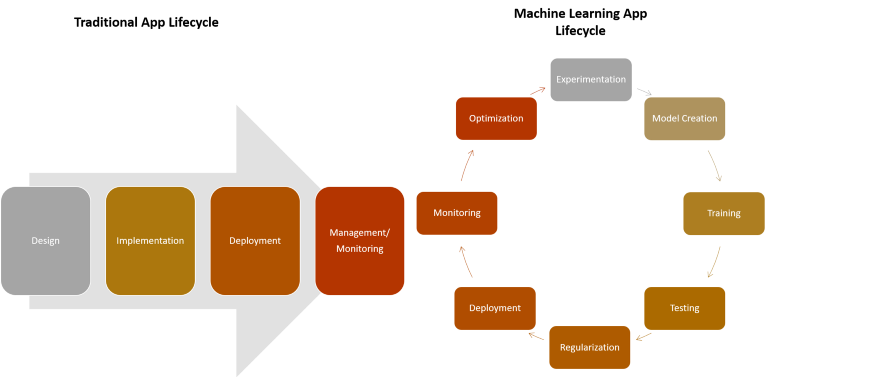
\includegraphics[scale=0.5]{images/ai_lifecycle.png}
\caption {Diferenças entre ciclos de vida de aplicações de software e aplicações de ML.~\citep{Rodriguez_2020}}
\label{fig:AILifeCycle}
\end{figure}

Em primeiro lugar, uma solução baseada em IA possui um ciclo de vida diferente de uma aplicação tradicional. Conforme ilustrado na Figura \ref{fig:AILifeCycle}, sua implementação envolve etapas como criação do modelo e treinamento, e sua fase de manutenção envolve otimizações devido aos novos volumes de dados que chegam em um determinado período de tempo, fazendo com que o modelo esteja sempre em constante mudança. Dessa forma, metodologias ágeis e ferramentas de integração contínua podem não cumprir seus objetivos de maneira ótima~\citep{Rodriguez_2020}.

\begin{figure}[h]
\centering
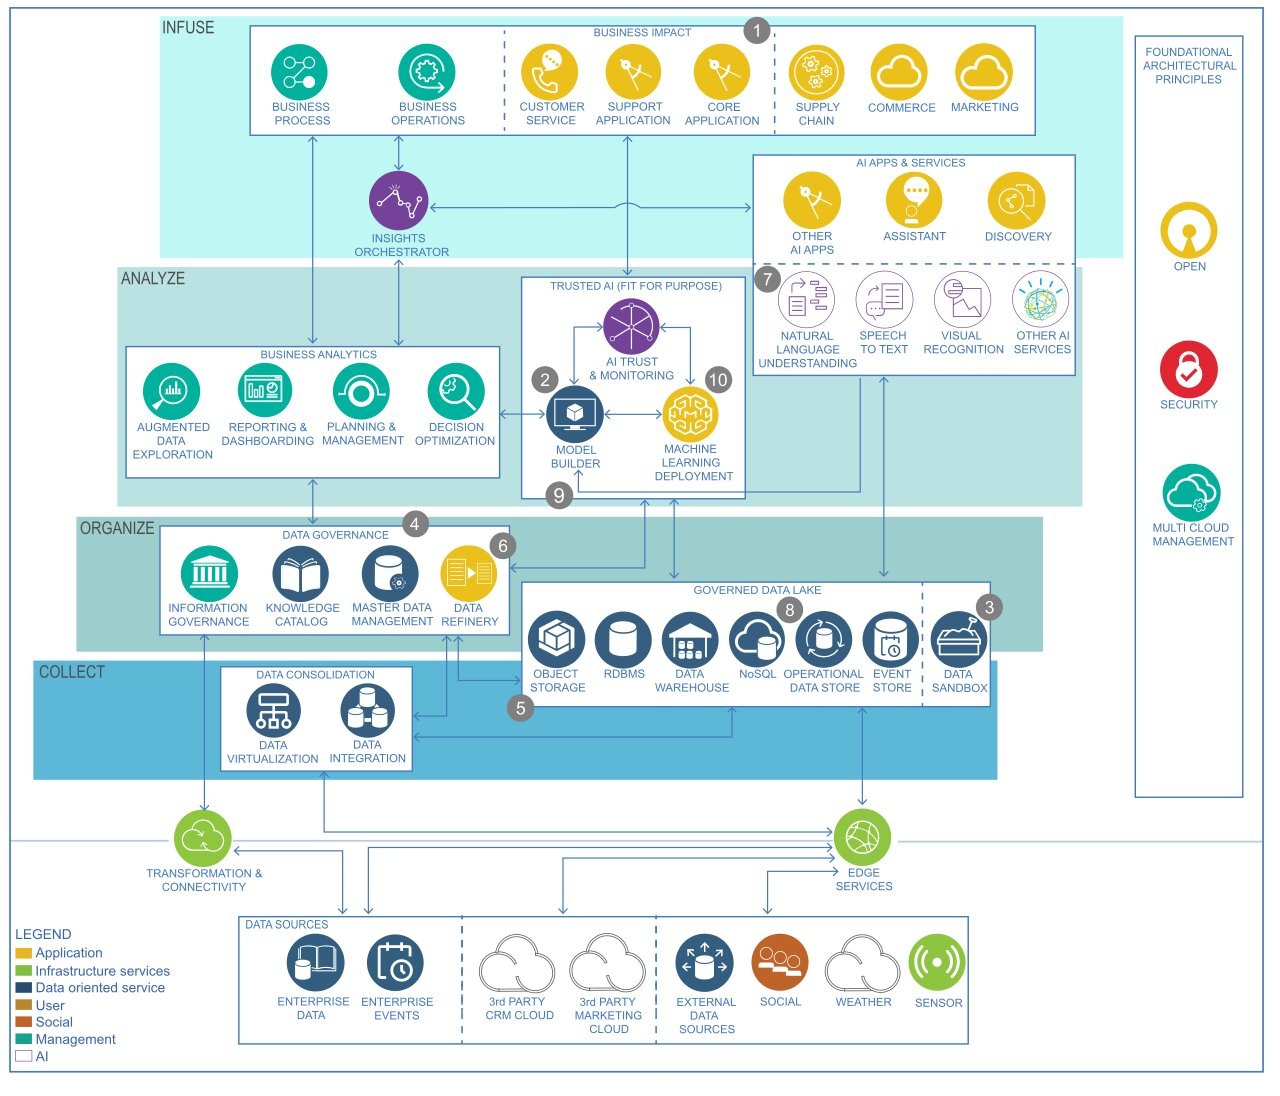
\includegraphics[scale=0.25]{images/ai-analytics-ref-diagram-analyze.jpg}
\caption {IBM Analytics and AI Reference Architecture.}
\label{fig:AIReferenceArchitecture}
\end{figure}

Além disso, o ciclo de vida da aplicação é apenas um dos pontos a se considerar, e as vezes o problema de uma aplicação pode estar em como o dado é obtido e disponibilizado. Um exemplo de arquitetura que generaliza todo o processo, desde a necessidade de negócio até o deploy do modelo de IA, é a IBM Analytics and AI Reference Architecture \citep{IBM_2021}, ilustrada na Figura \ref{fig:AIReferenceArchitecture}. Nela, são definidos os seguintes requisitos não-funcionais: Performance, estabilidade, segurança, escalabilidade, manutenibilidade e regulamentações de privacidade/\textit{compliance}, e pode ser classificada em 4 grupos principais envolvendo diversos tipos de processos e componentes:

\begin{itemize}
\item \textbf{Coleta:} Relaciona os processos de coleta, armazenamento e transformação de diversas fontes de dados, estruturadas ou não estruturadas, para determinados repositórios (\textit{Data Lakes}).
\item \textbf{Organização:} Relaciona os processos de organização e estruturação dos dados nos presentes nos \textit{Data Lakes} e necessários para o uso das aplicações que envolvem a análise dos dados. Dependendo do uso pode-se aplicar processos de Governança.
\item \textbf{Análise:} Relaciona os processos para desenvolvimento de aplicações de IA e relatórios após a organização dos dados para tomadas de decisão e uso de aplicações externas.
\item \textbf{Infusão:} Relaciona os processos de disponibilização desses dados e conhecimento obtidos na fase de análise para aplicações externas.
\end{itemize}

\section{Trabalhos Relacionados}

Os principais trabalhos encontrados envolvendo \textit{AI Explainability}, métricas de \textit{Fairness} e sua arquitetura vêm do time de engenharia do LinkedIn.~\citet{Geyik_2019} falam sobre as métricas utilizadas e os algoritmos implementados sobre ranqueamento dos dados.~\citet{Kenthapadi_2019} fala sobre como o conceito de \textit{Fairness} pode ser implementado em uma aplicação de IA, e mostra a arquitetura sobre ela, assim como outros estudos de caso~\citep{Kenthapadi_2020}.

No ramo de IA, muitos dos trabalhos desenvolvidos se referem a novas técnicas e modelos e poucos se referem realmente a arquitetura de um sistema. Entretanto, como os conceitos de \textit{AI Explainability} e métricas de \textit{Fairness} agem mais como extensões para construir modelos mais resilientes e não como novos paradigmas de modelagem, também podemos usar como referência arquiteturas de software já existentes e adaptá-las para já considerar estes conceitos desde sua base.

~\citet{Ballis_2017} propuseram em Stanford o projeto DAWN, que propõe uma série de ferramentas, \textit{frameworks} e uma arquitetura de referência para otimizar workflows de ML. Embora seja focada mais no processo de ML do que em XAI, uma de suas direções foca em elaborar interfaces para especialistas fora da área de ML e explicação de resultados e interpretações para humanos.

~\citet{Modi_2017} propuseram no Google o TFX, uma plataforma de ML para uso geral e baseada no TensorFlow, \textit{framework} do Google especializado em \textit{Deep Learning}. Ao integrar os componentes em uma plataforma, foram capazes de padronizar os componentes, simplificar a configuração da plataforma e reduzir o tempo de produção de meses para semanas, ao mesmo tempo que era fornecida estabilidade. Em um de seus trabalhos futuros, foi mencionada a necessidade de explicação das decisões e ações realizadas pelos modelos, conforme o uso de ML fosse se intensificando. O Google atualmente possui uma ferramenta para \textit{AI Explainability} em sua plataforma de computação em nuvem~\citep{Google_2021} possuindo métodos já implementados e disponibiliza explicações do modelo via metadados, mas nada foi encontrado em como isso era relacionado na arquitetura de um sistema real.

Uma outra arquitetura que é possível considerar e se basear é a FBFlow do Facebook~\citep{Dunn_2016}. Embora seja mais específica para a implementação e não possua qualquer menção a necessidades para explicação, o uso de DAGs (\textit{Direct Acyclic Graphs}) para a execução de um determinado processo ou \textit{workflow} é uma alternativa simples de ser implementada e interpretada pelos desenvolvedores, onde é possível conectar o método de ML juntamente com o cálculo de métricas e métodos de XAI para serem automatizados e organizados de forma simultânea.

\begin{table}[h]
\begin{center}
  \resizebox{\linewidth}{!}{%
  \begin{tabular}{ccccccccc}
    \toprule
    \multicolumn{2}{c}{\multirow{2}{*}{\bf Referências}} & \multicolumn{2}{c}{\multirow{2}{*}{\bf Descrição}} & \multicolumn{2}{c}{Arquitetura} & \multicolumn{3}{c}{Conceitos}\\
    \cmidrule{5-9}
%    \hline
    \multicolumn{4}{c}{} & \bf Arq. Referência & \bf Arq. Sistema & \bf XAI & \bf ML & \bf Fairness\\
    \midrule
    \multicolumn{2}{c}{Geyik et al., 2019} & \multicolumn{2}{c}{\makecell{Métricas utilizadas \\ Ranqueamento dos dados}} &  & \cmark &  & \cmark & \cmark\\[3ex]
%    \hline
    \multicolumn{2}{c}{Kenthapadi et al., 2019} & \multicolumn{2}{c}{Arquitetura/implementação de métricas de Fairness} &  & \cmark &  & \cmark & \cmark\\[2ex]
%    \hline
	\multicolumn{2}{c}{Kenthapadi et al., 2020} & \multicolumn{2}{c}{Desafios/lições sobre Explainable AI} &  & \cmark & \cmark & \cmark & \\[2ex]
%    \hline
    \multicolumn{2}{c}{\makecell{IBM Analytics and \\ AI Reference Architecture}} & \multicolumn{2}{c}{\makecell{Arquitetura de referência para Dados e ML}} & \cmark &  &  & \cmark & \\[3ex]
%    \hline
    \multicolumn{2}{c}{\makecell{Projeto DAWN - Stanford \\ (Ballis et al., 2017)}} & \multicolumn{2}{c}{\makecell{Ferramentas/Frameworks \\ Arquitetura de referência para ML}} & \cmark &  & Trab. Futuro & \cmark & \\[3ex]
%    \hline
    \multicolumn{2}{c}{\makecell{TFX - Google \\ (Modi et al., 2017)}} & \multicolumn{2}{c}{\makecell{Componentização/Padronização \\ Simplificação na implementação}} &  & \cmark & Trab. Futuro & \cmark & \\[3ex]
%    \hline
    \multicolumn{2}{c}{\makecell{FBFlow - Facebook \\ (Dunn, 2016)}} & \multicolumn{2}{c}{\makecell{Uso de DAGs para determinar \textit{workflow} \\ Execução/interpretação de processos de ML}} &  & \cmark &  & \cmark & \\
%    \hline
    \bottomrule
  \end{tabular}}
\end{center}
\end{table}

\section{Resultados Esperados e Desafios}

Espera-se obter como resultado desse projeto de mestrado uma proposta de arquitetura de software que acople os conceitos de \textit{Explainable AI} e métricas de \textit{Fairness} em uma solução de IA, com uma elaboração de caso de uso feito de acordo com as diretrizes obtidas neste projeto. Espera-se também que tal arquitetura se adeque independentemente de como os dados serão armazenados e processados.

O foco desse projeto não está necessariamente em obter resultados melhores em um modelo, e sim que a melhora dos resultados seja consequência de sua explicabilidade e de uma manutenção menos custosa. Espera-se também a elaboração e publicação de artigos em periódicos e eventos relacionados, relatando as experiências com o projeto e os resultados obtidos.

Por ser um campo bastante amplo e em constante evolução, este projeto terá limitações de escopo e voltará apenas para o aprendizado supervisionado, que é mais simples de ser explicado por já conhecermos suas entradas e saídas e por muitas soluções de IA serem treinadas com essa abordagem~\citep{Buolamwini_2018}. Entretanto, é esperado que este projeto contribua com diretrizes que possam se aplicar também a modelos não supervisionados e de aprendizado por reforço. 

Embora haja várias ferramentas e algoritmos baseados em \textit{Explainable AI}, as mesmas estão dispersas e há pouco material destinado a organizar estes tipos de ferramentas. Pretende-se solucionar isso com a elaboração de \textit{Checklists} e um caso de uso para estabelecer exemplos de desenvolvimento.

Embora as soluções de \textit{Explainability AI} ajudam a mesma a ser testável devido ao rastreamento do que está sendo notado para elaborar o resultado, é possível colocar como desafio que pontos estas soluções ajudam em específico. Como solução, é preciso realizar um estudo, assim como inclusão em documentação e exemplos no caso de uso.

Outro desafio está em como conectar os diferentes métodos utilizados com o método de ML e o conjunto de dados adequado. Para isso, componentes baseados na arquitetura MAPE-K~\citep{IBM_2005} podem ser úteis, podendo estabelecer uma base de conhecimento e estabelecer relações entre os métodos de forma adequada.

\section{Cronograma}

Conforme o programa de mestrado, o aluno realizará as disciplinas nos dois primeiros semestres, e durante o terceiro semestre participará do Programa de Estágio a Docência (PED) da Unicamp. Após a defesa do Exame de Qualificação de Mestrado (EQM), o aluno continuará a elaborar um estudo de caso e começará a redigir sua Dissertação. Ao final do segundo ano de projeto, será realizada a Dissertação de Mestrado do aluno.

As etapas que envolvem este projeto de Mestrado começarão no segundo semestre devido a uma desistência de orientação anterior do aluno, sendo possível ter uma prorrogação para um quinto semestre para a finalização do curso.

A Tabela abaixo mostra a estrutura do cronograma do projeto.

\begin{table}[h]
\begin{center}
  \resizebox{\linewidth}{!}{%
  \begin{tabular}{rcccccccc}
    \toprule
    \multicolumn{1}{c}{ } & \multicolumn{2}{c}{2020} & \multicolumn{4}{c}{2021}
    & \multicolumn{2}{c}{2022}\\
    \cmidrule{2-9}
%    \hline
    \bf Atividade & \multicolumn{2}{c}{\bf Semestre 1} & \multicolumn{2}{c}{\bf Semestre 2} & \multicolumn{2}{c}{\bf Semestre 3} & \multicolumn{2}{c}{\bf Semestre 4}\\
    \midrule
    Realização de disciplinas do IC & \multicolumn{2}{c}{\cmark} & \multicolumn{2}{c}{\cmark} & \multicolumn{2}{c}{ } & \multicolumn{2}{c}{ }\\
    %    \hline
    Estudo e catálogo de artigos & \multicolumn{2}{c}{ } & \multicolumn{2}{c}{\textbullet} & \multicolumn{2}{c}{} & \multicolumn{2}{c}{}\\
%    \hline
    Revisão bibliográfica & \multicolumn{2}{c}{ } & \multicolumn{2}{c}{\textbullet} & \multicolumn{2}{c}{\textbullet} & \multicolumn{2}{c}{\textbullet}\\
%    \hline
    Elaboração de caso de uso & \multicolumn{2}{c}{ } & \multicolumn{2}{c}{ } & \multicolumn{2}{c}{\textbullet} & \multicolumn{2}{c}{\textbullet}\\
%    \hline
    Qualificação & \multicolumn{2}{c}{ } & \multicolumn{2}{c}{\textbullet} & \multicolumn{2}{c}{ } & \multicolumn{2}{c}{ }\\
%    \hline
    Escrita da dissertação & \multicolumn{2}{c}{ } & \multicolumn{2}{c}{ } & \multicolumn{2}{c}{\textbullet} & \multicolumn{2}{c}{\textbullet}\\
%    \hline
    Realização do PED & \multicolumn{2}{c}{ } & \multicolumn{2}{c}{ } & \multicolumn{2}{c}{\textbullet} & \multicolumn{2}{c}{ }\\
%    \hline
    Publicação de artigo & \multicolumn{2}{c}{ } & \multicolumn{2}{c}{ } & \multicolumn{2}{c}{ } & \multicolumn{2}{c}{\textbullet}\\
%    \hline
    Defesa & \multicolumn{2}{c}{ } & \multicolumn{2}{c}{ } & \multicolumn{2}{c}{ } & \multicolumn{2}{c}{\textbullet}\\
    \bottomrule
  \end{tabular}}
\end{center}
\end{table}
% As referências:
\bibliographystyle{plainnat}
\bibliography{project}
\end{document}
